\documentclass{iiththesis}
\usepackage{caption}
\usepackage{subcaption}
\usepackage{multirow}
\usepackage[normalem]{ulem}
\useunder{\uline}{\ul}{}

\newcommand{\vk}[1]{\textcolor{orange}{\textbf{VK:}#1}}
\newcommand{\ra}[1]{\textcolor{blue}{\textbf{RA:}#1}}
\newcommand{\urk}[1]{\textcolor{red}{\textbf{URK:}#1}}

\newcommand{\fixme}[1]{\textcolor{red}{\textbf{URK:}#1}}

% \usepackage{hyperref}
\book{Thesis}
\title{Applying Machine Learning to Compiler and Programs}
\degree{Master of Technology}
\department{Computer Science and Engineering}
\submitted{\today}
\author{Rohit Aggarwal}
\adviser{Dr. Ramakrishna Upadrasta}
\addradviser{Dept. of Computer Science and Engineering \\ IITH}
\chair{Dr. Rogers Mathew}
\addrchair{Dept. of Computer Science and Engineering \\ IITH}
% \external{----------}
% \addrexternal{Dept. of Chem Eng \\ IITM}
\external{Dr. Saurabh Joshi}
\addrexternal{Dept. of Computer Science and Engineering \\ IITH}
\internal{Dr. Sathya Peri}
\addrinternal{Dept. of Computer Science and Engineering \\ IITH}
% \coguide{----------}
% \addrcoguide{Dept. of Chem Eng \\ IITH}


% \label{acks}
\acknowledgements{

I Thanks you for using this!

}

\dedication{\begin{center}
Dedicated to \\\textbf{\textit{my Family and Friends}}
\end{center}}
\abstract{

Here goes the abstract.

}


\renewcommand{\bibname}{References}
% \newcommand{\irtovec}{{\textsc{IR2Vec}}\xspace}
\begin{document}
\chapter{Introduction}
\label{chap:intro}


In the current days, Machine Learning (ML) is being used in many domains for achieving the tasks which were previously very hard, or the known algorithm(s) were either not efficient, or had poor success rate. 


There are many types of ML algorithms with different kinds of capability and usage. 
These are broadly divided into categories like supervised learning, unsupervised learning, semi-supervised learning etc. Supervised learning problems are either classification or Regression. Classification is a task in which the model predicts the tag or label from the given labels for a given data point. Tagging the image and sentiment analysis are examples of the classification. 
In regression, the model predicts the value between an interval. Price of the house, Pollution growth-decline prediction are famous examples for regression.

	
Most of the current success of ML is due to the success of Deep Learning. Deep learning (DL) is a type of ML in which a neural network is used as a function approximator. Neural network is the network of neuron. A neuron is the basic unit of a neural network.\vk{Seems to be inaccurate}.  The major breakthrough was the AlexNet~\cite{alexnet:NIPS_2012} which came into prominence when they won the ImageNet challenge by presenting results that improved by a large margin the results compared to the previous state of the art.
	
\paragraph{DL, Program Representations and Applications:}
Recently, there are several works that focus on program representations that are given as inputs for DL. The learnt inputs are used for several important  applications: program tagging, summarization, vulnerability detection, and others from the software engineering domain. Device mapping and thread coarsening are examples of two applications from the code-optimization domain.

\paragraph{LLVM Compiler:}
LLVM~\cite{Lattner:2004:llvm} is a modern, open-source compiler tool-chain. It supports many frontend languages like C, C++, Haskel, Go, Swift, etc. and backends like x86, ARM, AMDGPU, NVIDIA, etc. It has very rich intermediate representation (IR) on which many optimizations can be easily implemented and applied without much difficulty.
	    
\paragraph{Program Representations using LLVM}
We have worked on the program representation for LLVM IR. We can generate the Instruction level, function level, and program level embedding. These embeddings can be used in many software engineering and optimization tasks depending on the necessity.


    	


\paragraph{Overview of this thesis:}
The following is a brief overview of this thesis:

\begin{itemize}
    \item In \textit{Chapter \ref{chap:ch2}}, we will begin with discussing the background about program encodings and in particular about IR2Vec encoding~\cite{IR2Vec}. 
    Then, we will discuss about applying this encoding to Thread Coarsening task. The result of this application is prediction of Thread Coarsening Factor; our results improve from the other state-of-the-art works.
    
    \item In \textit{Chapter \ref{chap:ch3}}, we will discuss about performing Algorithm Recognition with IR2Vec in both supervised and few-shot setting. \vk{not unsupervised}
    We have written a program classification model using TensorFlow~\cite{tensorflow_USENIX2016} and PyTorch~\cite{pytorch} for the unseen classes of algorithms.	

    \item In \textit{Chapter \ref{chap:ch4}}, we have done a case study on an approach to achieve optimal-distribution using fusion and inline
    
    \item In \textit{Chapter \ref{chap:ch5}}, we will discuss about Machine learning framework for Register Allocation 
    
    \item  In \textit{Chapter~\ref{chap:conclude}}, we will conclude our work.
    
    \fixme{AAA AAA}
    
    

\end{itemize}
\chapter{Applying IR2Vec to Thread Coarsening}
\label{chap:ch2}


\section{Introduction to IR2Vec}
% \subsection{Overview}
\vk{Should say what is IR2Vec here}
The overview of the proposed methodology is shown in Fig.~\ref{fig:IR2Vec-Overview}. Instructions in IR can be represented as an Entity-Relationship Graph, with the instruction entities as nodes, and the relation between the entities as edges. A translational learning model is used to learn these relations. The output of this learning is a dictionary containing the embeddings of the entities and is called \textit{Seed embedding vocabulary}. 

\begin{figure}[t]
    \centering
    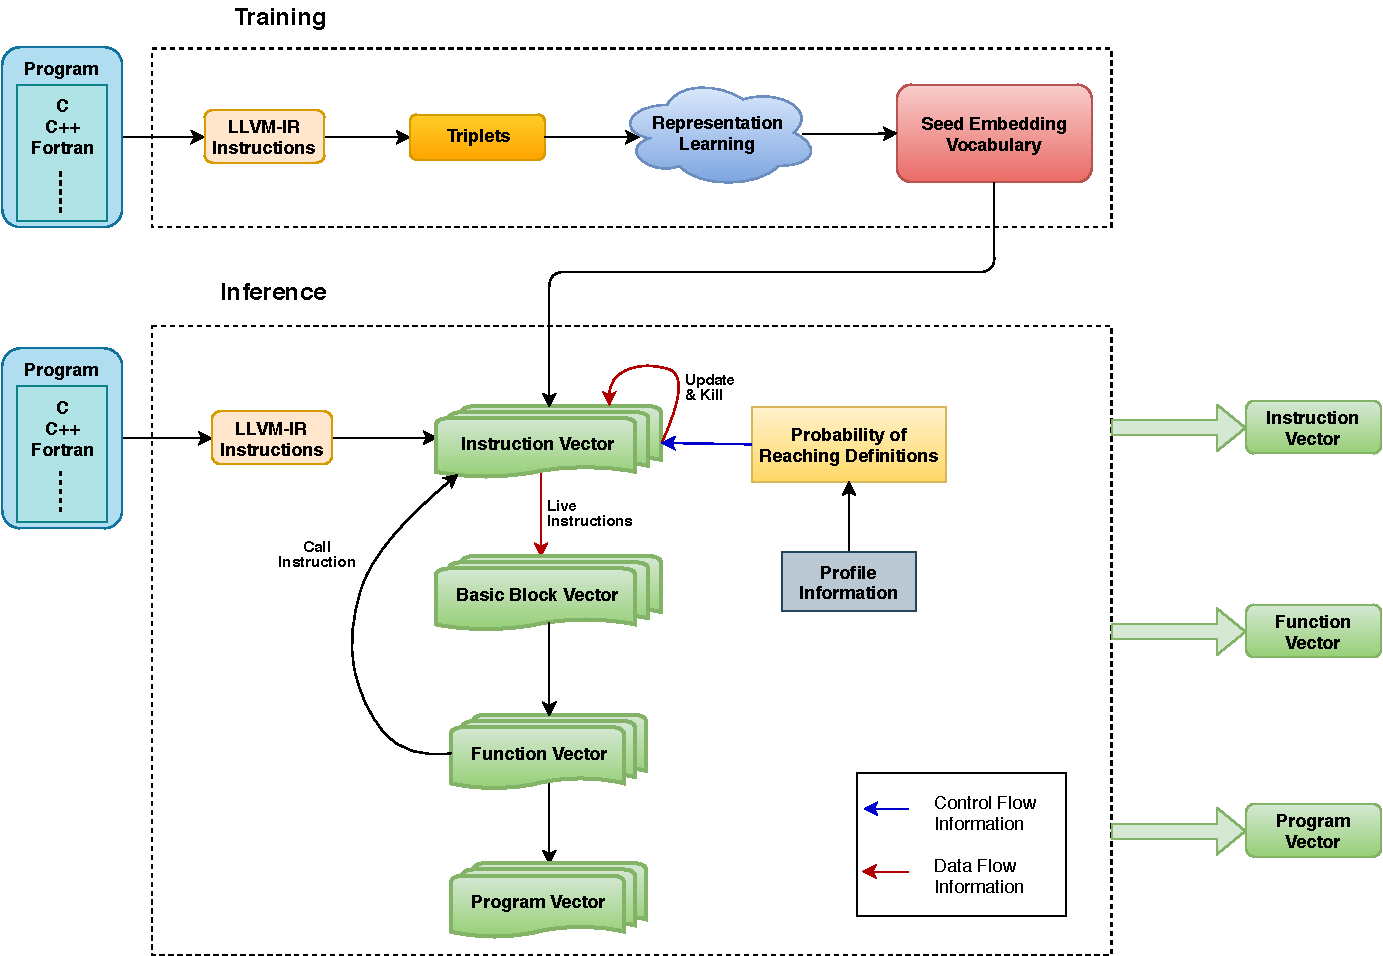
\includegraphics[scale=0.5]{figures/chapter-2/flow.pdf}
    \caption{Overview of IR2Vec infrastructure}
     \label{fig:IR2Vec-Overview}
\end{figure}

The above dictionary is looked up to form the embeddings at various levels of the input program. 
At the coarsest level, instruction embeddings are obtained just by using the \textit{Seed embedding vocabulary}. We call such encodings as \textit{Symbolic} encodings.
We use the \textit{Use-Def} and \textit{Reaching definition}~\cite{Hecht:1977:FAC:540175, muchnick1997advanced} information to form the instruction vector for \textit{Flow-Aware} encodings. 

The instructions which are \textit{live} are used to form the \textit{Basic block Vector}  using the flow analysis information. The vector to represent a function is obtained by using the basic block vectors of the function. The \textit{Code vector} is obtained by propagating the vectors obtained at the function level with the \texttt{call graph} information.
\section{Thread Coarsening Task}
Thread coarsening~\cite{Volkov-Demmel-10.5555/1413370.1413402} is the process of increasing the work done by a single thread by fusing two or more concurrent threads. Thread coarsening factor corresponds to the number of threads that can be fused together. Selection of an optimal thread coarsening factor can lead to significant improvements~\cite{Magni-SC13-DBLP:conf/sc/MagniDO13} in the speedups on GPU devices and a naive coarsening would lead to a substantial slowdown.

A thread coarsening factor of a kernel that gives the best speedup on a GPU could give the worst performance with the same coarsening factor on another device (either within or across vendors) because of the architectural characteristics of the device~\cite{magni2014automatic, Stawinoga-10.1145/3194242}. For example, \texttt{nbody} kernel, which has a higher degree of Instruction Level Parallelism, can be better exploited by VLIW based AMD Radeon than SIMD based AMD Tahiti~\cite{magni2014automatic}.

\subsection{Dataset} 
In this experiment, we follow the experimental setup proposed by Magni et al.~\cite{magni2014automatic} to predict the optimal thread coarsening factor---among $\{1,2,4,8,16,32\}$---for a given kernel specific to a GPU device. Even for this experiment, we use the dataset provided by Ben-Nun et al.~\cite{ncc}. It consists of about 68 datapoints from 17 OpenCL kernels on 4 different GPUs -- AMD Radeon 5900, AMD Tahiti 7970, NVIDIA GTX 480 and NVIDIA Tesla K20c.
These kernels are collectively taken from AMD SDK, NVIDIA SDK and Parboil benchmarks.
A datapoint consists of the kernel and its runtime corresponding to each thread coarsening factor on a particular GPU device.

\subsection{Experimental Setup}
Even for this task, we use gradient boosting classifier instead of LSTMs and RNNs to predict the coarsening factor for the four GPU targets. For this experiment, we set the learning rate as 0.05 with 140 decision stumps with 1 level, as the number of data points in the dataset is very low. We use ten-fold cross-validation for measuring the performance.

\begin{table}[h]
\centering
  \caption{\% improvement in speedup obtained by Flow-Aware encodings when compared to the other methods}
%   \vspace*{-\baselineskip}
  \label{tab:predictionSpeedup-tc}    \small
  \begin{tabular}{p{2.5cm}p{1.9cm}p{1.6cm}p{1.5cm}p{2.2cm}p{1.5cm}}
    \hline
    \textbf{Architecture} & \textbf{Magni et al. \cite{o2013portable-grewe}} & \textbf{DeepTune \cite{cummins2017end2end}} & \textbf{DeepTune-TL \cite{cummins2017end2end}} & \textbf{inst2vec \cite{ncc}}\footnotemark  & \textbf{IR2Vec  Symbolic}\\
    \hline
    \textbf{AMD Radeon 5900} & 27.66\% & 5.26\% & 5.26\% & 4.35\% & -- \\
    \textbf{AMD Tahiti 7970} & 25.41\% & 29.37\% & 36.56\% & 18.17\% & 2.08\% \\
    \textbf{NVIDIA GTX 480} & 45.31\% & 25.21\% & 18.89\% & 23.89\% & 3.98\%\\
    \textbf{NVIDIA Tesla K20c} & 52.84\% & 15.41\% & 11.98\% & 11.98\% & 0.18\%\\
\hline
\end{tabular}
\end{table}
\footnotetext{As per the results given in the NCC paper~\cite{ncc}, inst2vec-imm achieves a (arithmetic) mean of $ 1.28\times$, $ 1.18\times$, $ 1.11\times$ and $1\times$ speedup on AMD Radeon, AMD Tahiti, NVIDIA GTX and NVIDIA Tesla; whereas our \textit{Flow-Aware} encodings achieve a (arithmetic) mean of $ 1.25\times$, $ 1.3\times$, $ 1.26\times$ and $ 1.16\times$ respectively.}

\subsubsection{Speedups}
In Fig.~\ref{fig:tcSpeedup}, we show the speedups achieved by our encodings and earlier works on four different platforms -- AMD Radeon HD 5900, AMD Tahiti 7970, NVIDIA GTX 480 and NVIDIA Tesla K20c. 

On AMD Radeon, both of our encodings achieve a speedup of $ 1.2\times$ when compared to the state-of-the-art speedup of $ 1.15\times$ and $ 1.14\times$ achieved by inst2vec~\cite{ncc} and DeepTune model with transfer learning (DeepTune-TL)~\cite{cummins2017end2end}.
In AMD Tahiti, \textit{Flow-Aware} encodings achieve a speedup of $ 1.23\times$; \textit{Symbolic} encoding achieves a speedup of $ 1.2\times$, whereas the earlier works by DeepTune-TL and inst2vec achieve a speedup of $ 0.9\times$ and $ 1.04\times$ respectively. In Tab.~\ref{tab:predictionSpeedup-tc}, we show the percentage improvement of speedup obtained by \textit{Flow-Aware} encodings over other methodologies. From the table, we can infer that \textit{Flow-Aware} gives better results for every architecture when compared to the other methods. 

% \begin{figure}
%     \centering
%     \begin{tabular}{@{}c@{}}
%         \includegraphics[scale=0.55, width=\textwidth]{figures/TC/radeon.pdf}
%     \end{tabular}
%     % \vspace{-5cm}
%     \begin{tabular}{@{}c@{}}
%         \includegraphics[scale=0.55, width=\textwidth]{figures/TC/tahiti.pdf}
%     \end{tabular}
%     \begin{tabular}{@{}c@{}}
%         \includegraphics[scale=0.55, width=\textwidth]{figures/TC/gtx.pdf}
%     \end{tabular}
%     \begin{tabular}{@{}c@{}}
%         \includegraphics[scale=0.55, width=\textwidth]{figures/TC/tesla.pdf}
%     \end{tabular}
%     \caption{Plot showing the speedups achieved by predicted coarsening factors by various methods}
%     % \vspace*{-\baselineskip}
%     \label{fig:tcSpeedup}
%      \vspace*{-0.4cm}
% \end{figure}

% \begin{figure}
%     \centering
%     \begin{tabular}{@{}c@{}}
%         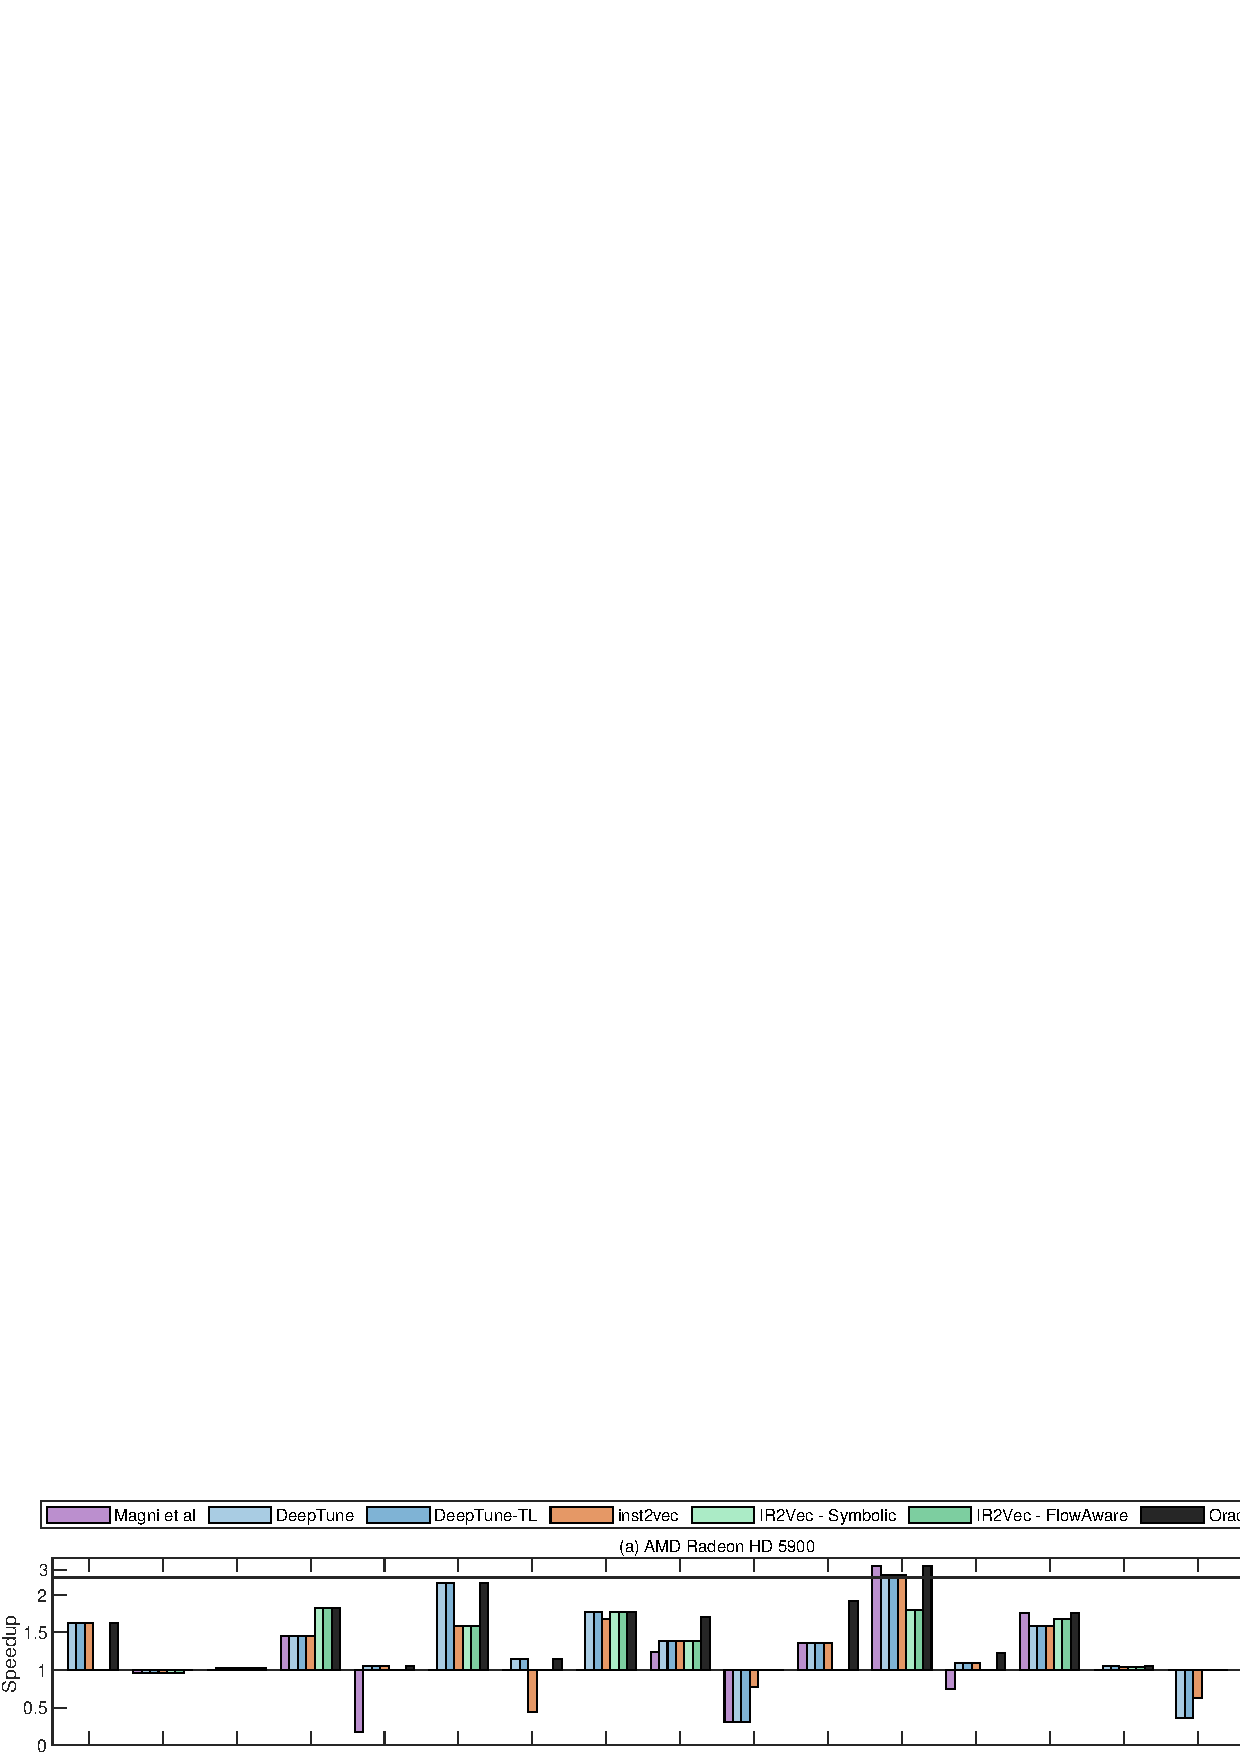
\includegraphics[scale=0.8, width=\textwidth]{figures/TC/new/radeon1-crop.pdf}
%     \end{tabular}
%     % \vspace{-5cm}
%     \begin{tabular}{@{}c@{}}
%         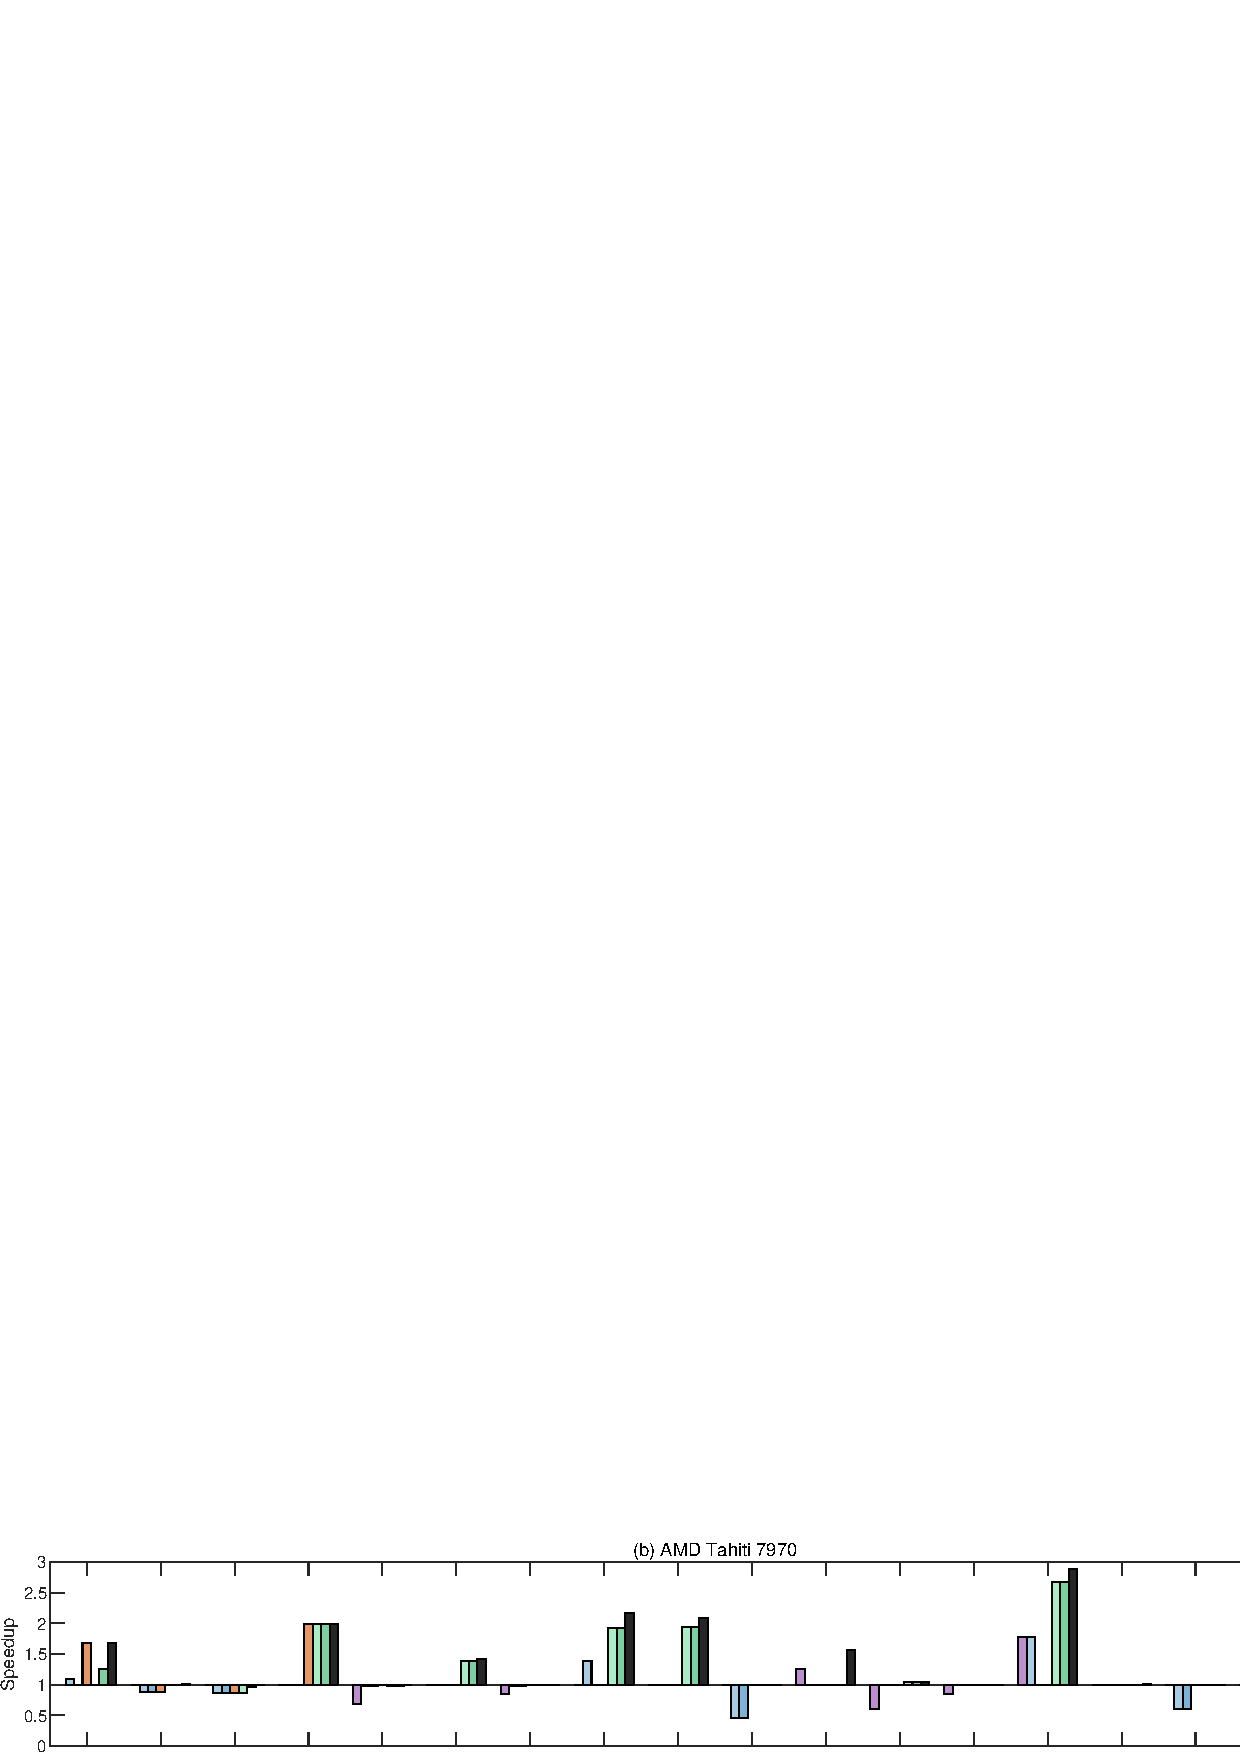
\includegraphics[scale=0.8, width=\textwidth]{figures/TC/new/tahiti2-crop.pdf}
%     \end{tabular}
%     \begin{tabular}{@{}c@{}}
%         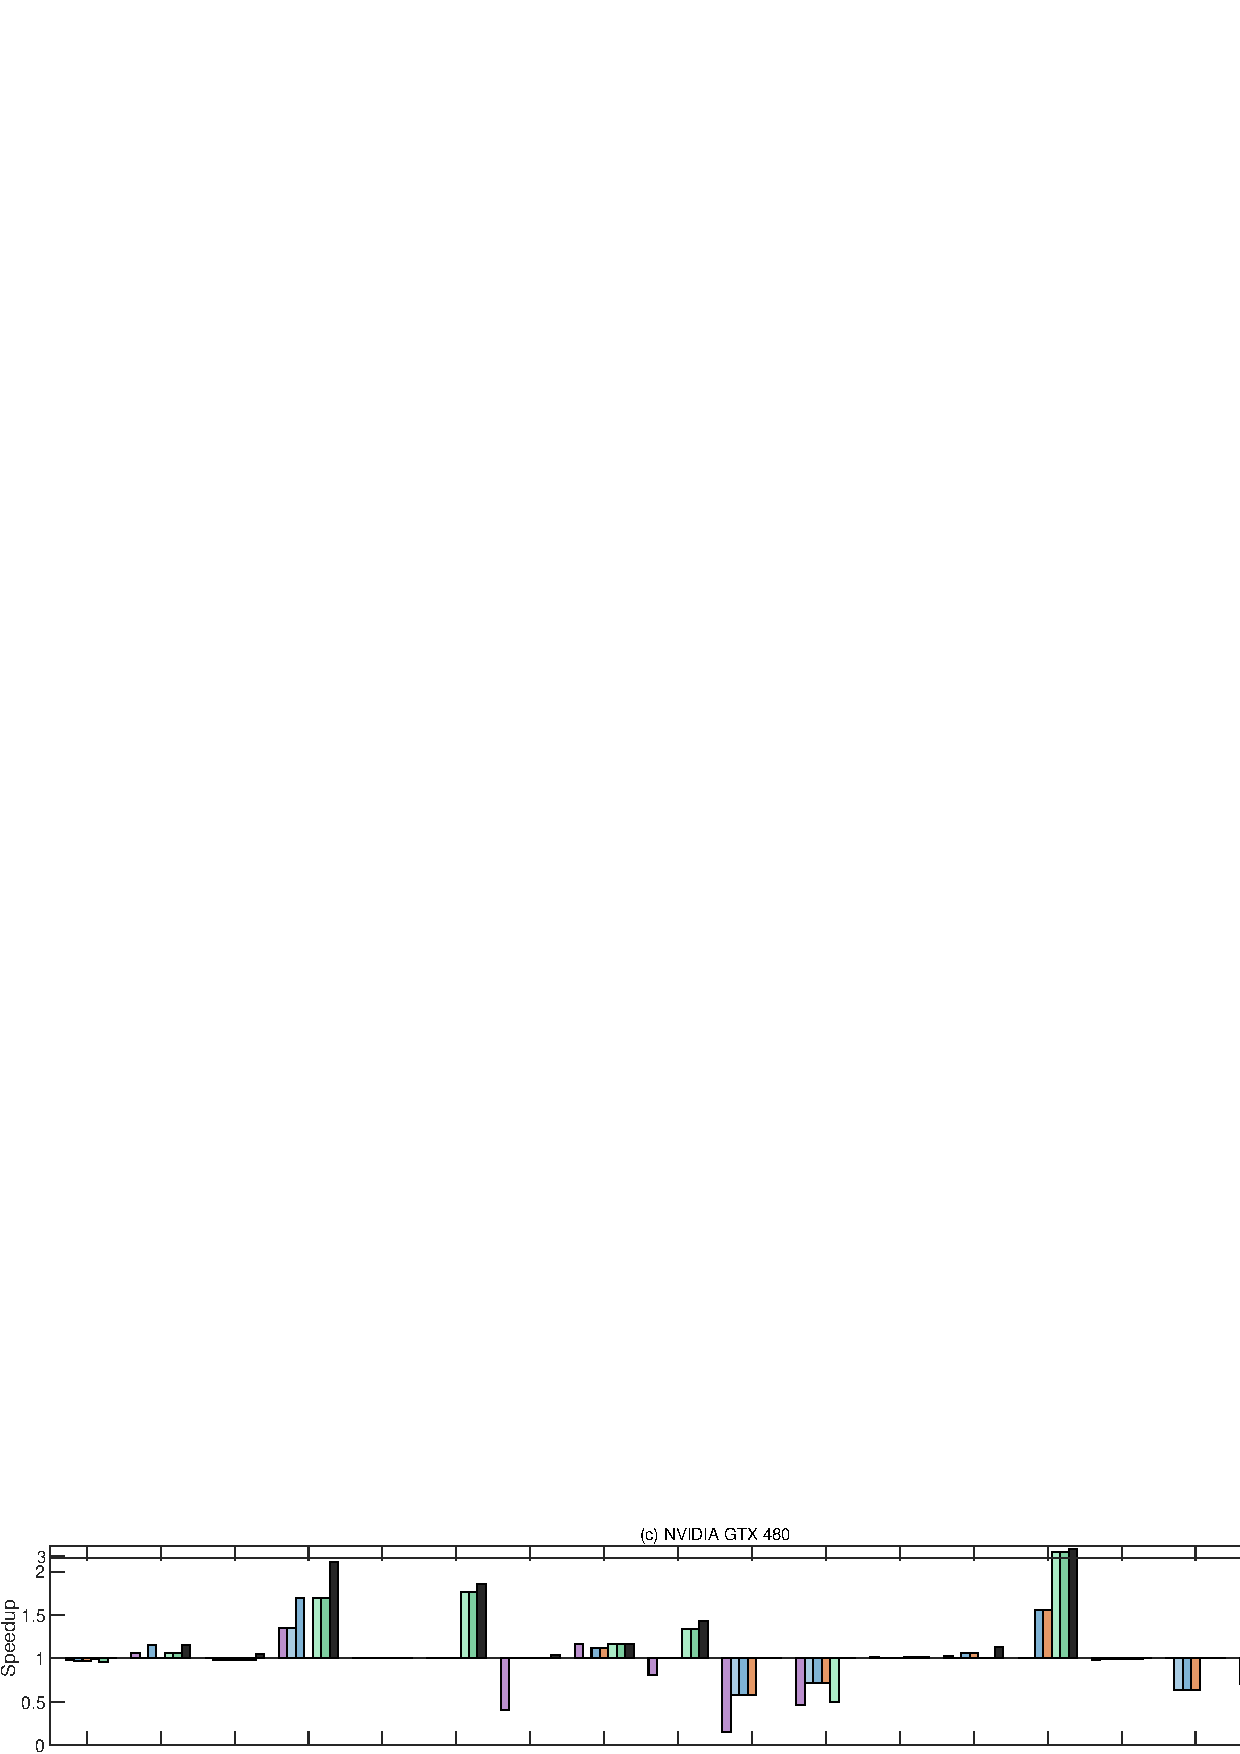
\includegraphics[scale=0.8, width=\textwidth]{figures/TC/new/gtx-crop.pdf}
%     \end{tabular}
%     \begin{tabular}{@{}c@{}}
%         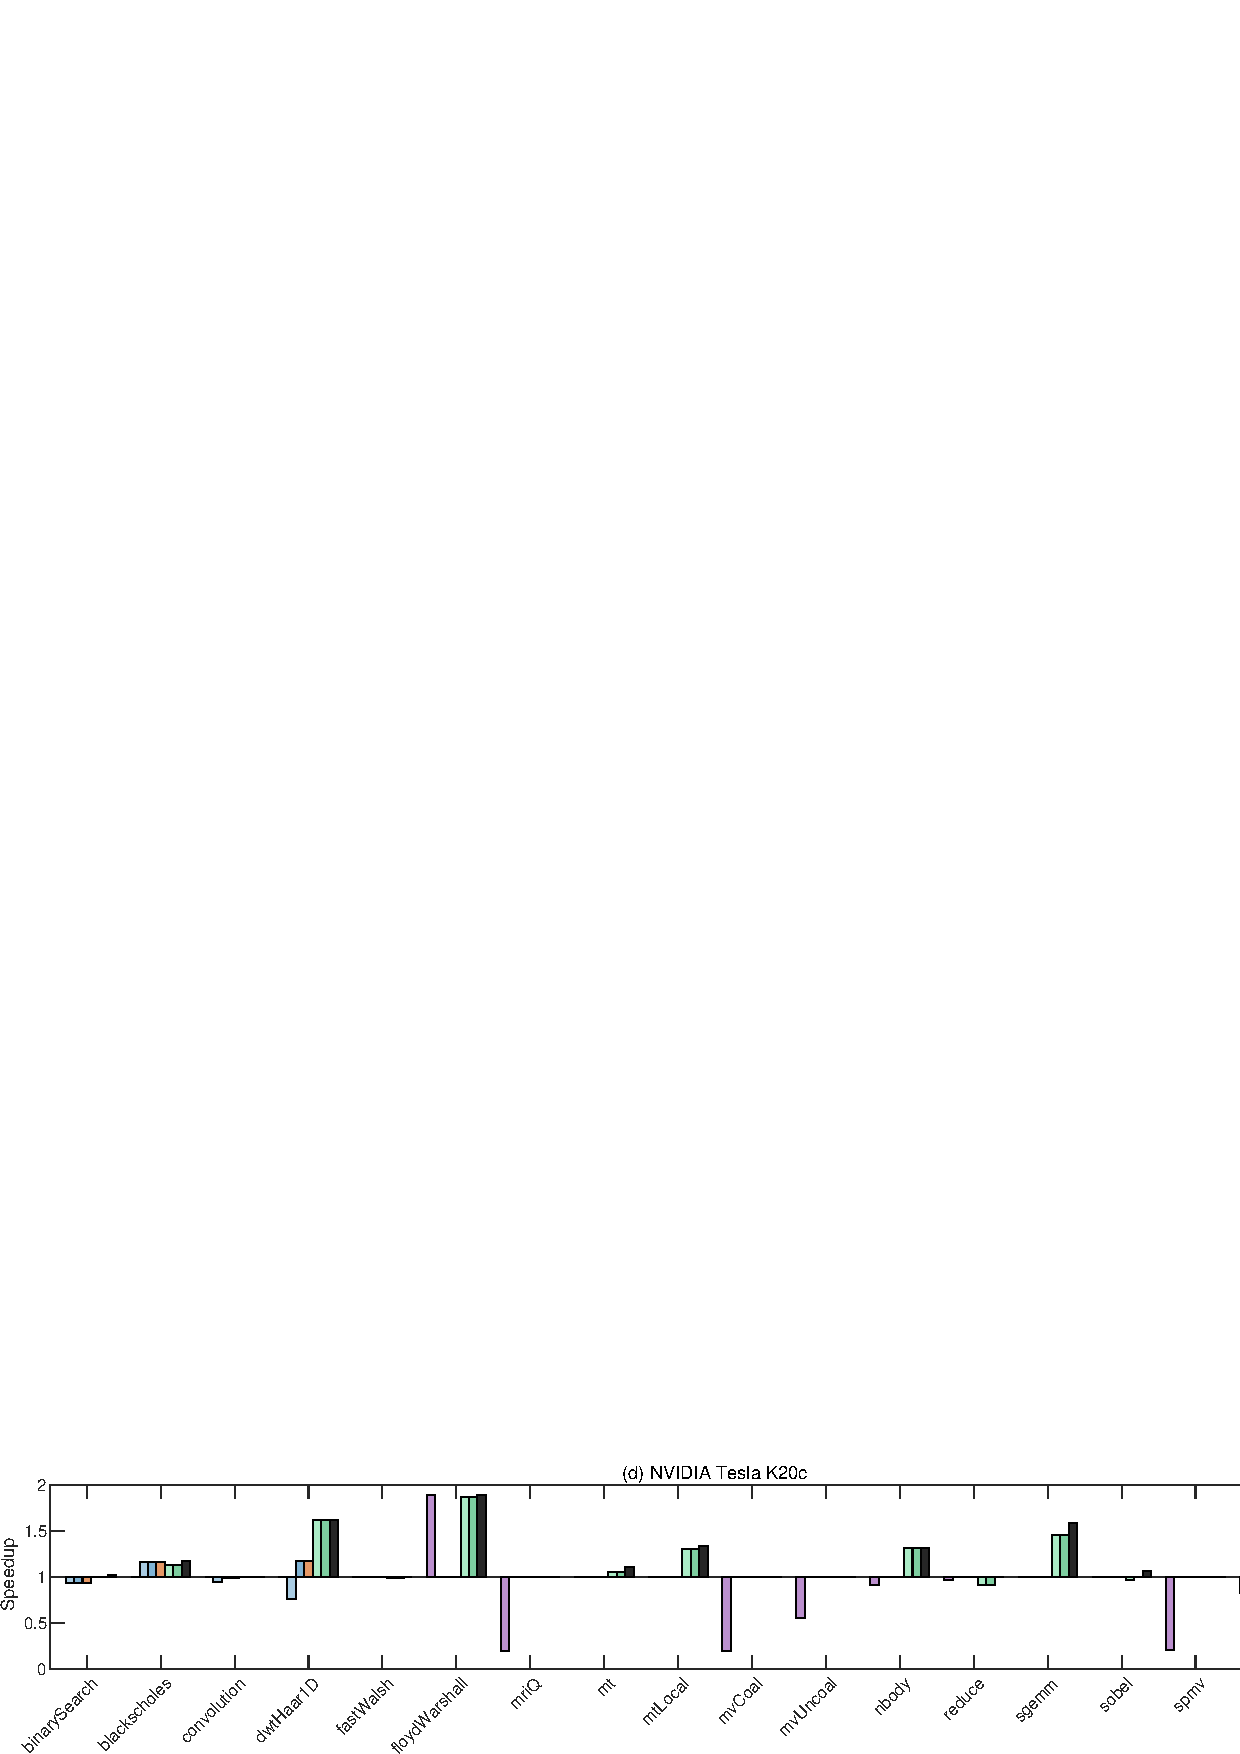
\includegraphics[scale=0.8, width=\textwidth]{figures/TC/new/tesla2-crop.pdf}
%     \end{tabular}
%     \caption{Plot showing the speedups achieved by predicted coarsening factors by various methods}
%     % \vspace*{-\baselineskip}
%     \label{fig:tcSpeedup}
%      \vspace*{-0.4cm}
% \end{figure}

\begin{figure}
    \centering
    \begin{tabular}{@{}c@{}}
        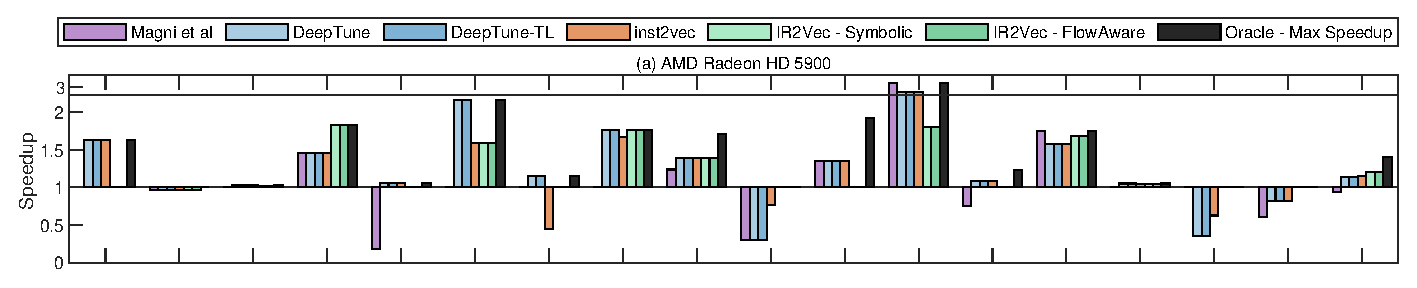
\includegraphics[scale=0.8, width=\textwidth]{figures/TC/radeon1-crop.eps}
    \end{tabular}
    % \vspace{-5cm}
    \begin{tabular}{@{}c@{}}
        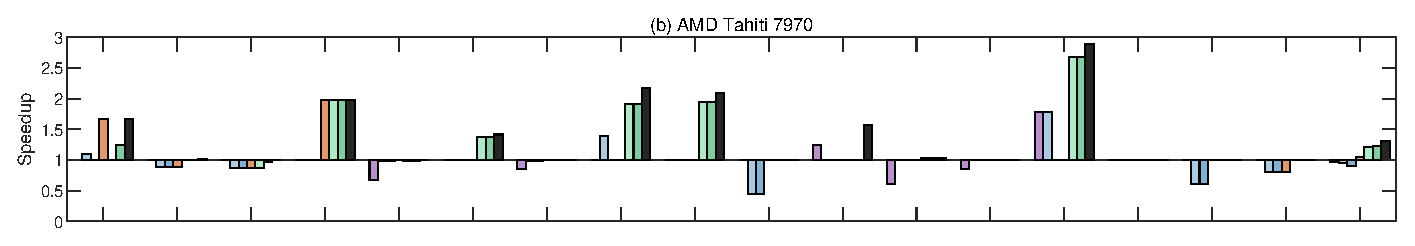
\includegraphics[scale=0.8, width=\textwidth]{figures/TC/tahiti2-crop.eps}
    \end{tabular}
    \begin{tabular}{@{}c@{}}
        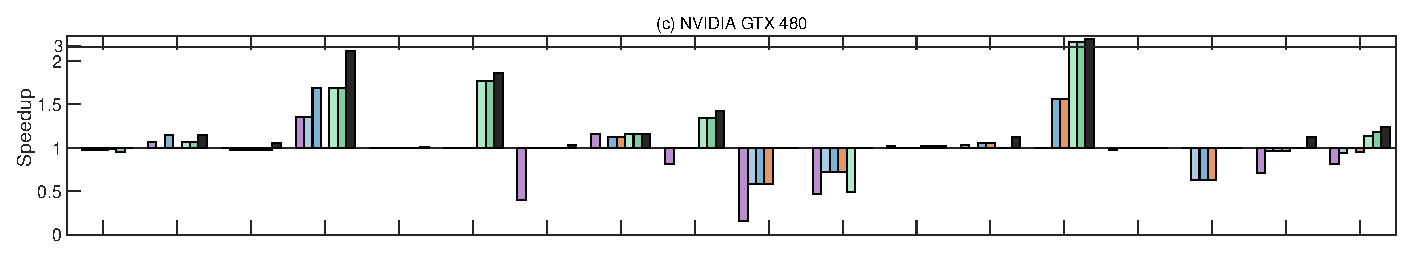
\includegraphics[scale=0.8, width=\textwidth]{figures/TC/gtx-crop.eps}
    \end{tabular}
    \begin{tabular}{@{}c@{}}
        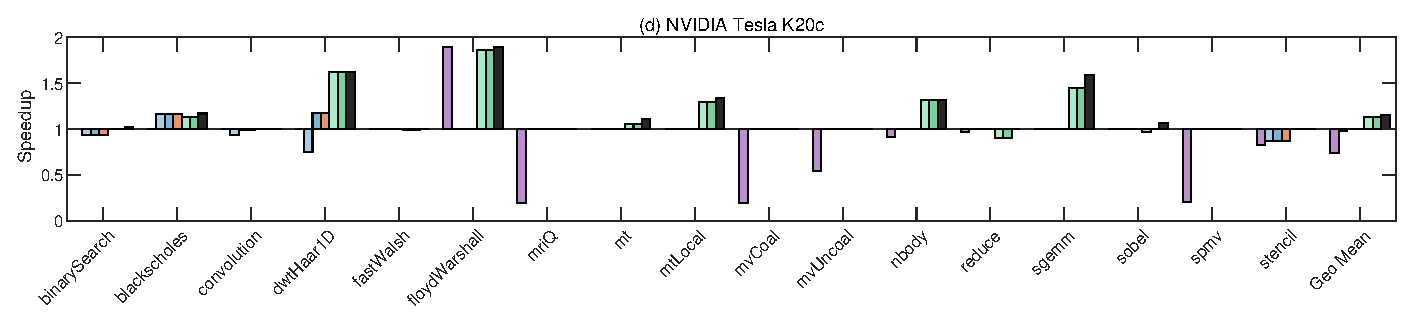
\includegraphics[scale=0.8, width=\textwidth]{figures/TC/tesla2-crop.eps}
    \end{tabular}
    \caption{Plot showing the speedups achieved by predicted coarsening factors by various methods}
    % \vspace*{-\baselineskip}
    \label{fig:tcSpeedup}
     \vspace*{-0.4cm}
\end{figure}


We are the \textit{first ones} to achieve a positive speedup on NVIDIA GTX 480; our \textit{Flow-Aware} and \textit{Symbolic} encodings obtain a speedup of $ 1.18\times$ and $ 1.13\times$ respectively when compared to $ 0.95\times$ and $ 0.99\times$ speedup achieved by inst2vec and DeepTune-TL. 
We get a speedup of $ 1.13\times$ with both of our proposed encodings on NVIDIA Tesla K20c. In contrast, DeepTune-TL and inst2vec obtain a speedup of $ 1.01\times$ on this platform.

On average, it can be seen that both encodings outperform the earlier methods for prediction of the thread coarsening factor on all the four platforms under consideration. 

\subsubsection{Slowdown}  Magni et al.~\cite{magni2014automatic} observe that \texttt{spmv} and \texttt{mvCoal} kernels have irregular dependences that causes a poor response to coarsening, and hence no performance improvement for them is possible.
For these kernels, IR2Vec obtains the baseline speedup \textit{without} resulting in a slowdown. In contrast, the earlier models result in negative speedups (Deeptune results in a slowdown upto $0.36$ $\times$ in AMD Radeon and inst2vec results in a slowdown of upto $0.63$ $\times$ in AMD Radeon and NVIDIA GTX). 
The same argument applies for \texttt{stencil} kernel (an iterative Jacobi stencil on 3D-grid), where the coarsening leads to slowdown (except in NVIDIA GTX), while IR2Vec still obtain the baseline speedup.

When compared to the other methods, we obtain the best speedup on about 70\% of the kernels on all platforms. 
It can be observed that the \textit{Flow-Aware} encodings \textit{rarely lead to slowdowns}; this happens in only 8/68 cases (17 benchmark-suits, across 4 platforms), even on these eight cases, the speedup is still close---within 10\%---of the baseline. 
Whereas, predictions by inst2vec and DeepTune-TL result in a slowdown in 18 and 21 cases.
We believe that this is because of the flow information associated with the obtained vectors.

\paragraph{Training}
Our model takes lesser time of $\approx$10 seconds for training when compared to $\approx$11 hours of training time needed by DeepTune-TL and $\approx$1 hour of training time needed (and 77K and 69K parameters used) by DeepTune and NCC approaches. 
This results in $\approx 360\times$--$3960\times$ reduction of training time, and again, achieving good speedups. 


\section{Conclusion}\label{sec:tc:conclusion}
We are able to achieve better results with respect to the prior work in term of both accuracy. Additionaly, the training time of the model is far better then the others.
\chapter{Algorithm Recognition}
\label{chap:ch3}

\section{Supervised Learning}
Supervised Learning is the field of machine learning in which the model is trained against known label or tags. The model for a given data point can't predict any thing not mentioned in the vocabulary. There are some fixit numbers of label for a machine learning task.

\subsection{Background}
In case of the image classification, there is a image dataset and each image is labeled. We run the training using the given images as the input and predict the image label. Given the true value and predicted value, we calculate the loss with is used to generate gradient.

\subsection{Methodology}
On the similarly ground, We are trying to do algorithm recognition. Here given the bunch of the program, we want to predict to give algorithm class the program belong to.

We developed an classifier in TensorFlow which can classify the program respectively. 
\subsubsection{DataSet}
We have selected the POJ-104 dataset\ref{} for our experiments. It has 104 type of different program which acts like class or label and each class has approximately ~500 programs. We have splitted this dataset into 3:1:1(training:testing:validation).

\subsection{Embedding Generation}
I have used IR2Vec to generate the embedding for the programs. For each program, we get a 300 dimension vector and it's corresponding label.

\subsection{Model Architecture}
The first input layer expects a 300-dimension vector which is followed by simple three layered Multi-Level Precptron(MLP) with a softmax layer for output. The Categorical cross entropy Loss is used as the loss function and Adam as the optimizer. The whole training run for 100 epochs.

\subsection{Results}
% Table~\ref{tab-acc} rather than table~\ref{tab-acc}.
\begin{table}[h]
\begin{tabular}{l l l l}
\hline
Percentage & TBCNN & inst2vec &  Ours\\
\hline
Accuracy(\%) & 94 & 94.83 & 96.2 \\
\hline
\end{tabular}
\centering
\caption{Compare the accuracy percentage.}
\label{tab-acc}
\end{table}

\subsection{Visual Technique}
As mentioned above have 300 dimension vector and it reduce it's dimension to 2 dimensions using t-SNE\cite{}. Points which are similar to each other meant to be near to each other. The effectiveness of the encoding different instance to time during training is shown.

\begin{figure}[h]
    % \centering
\begin{subfigure}[b]{0.3\textwidth}
%   \centering
  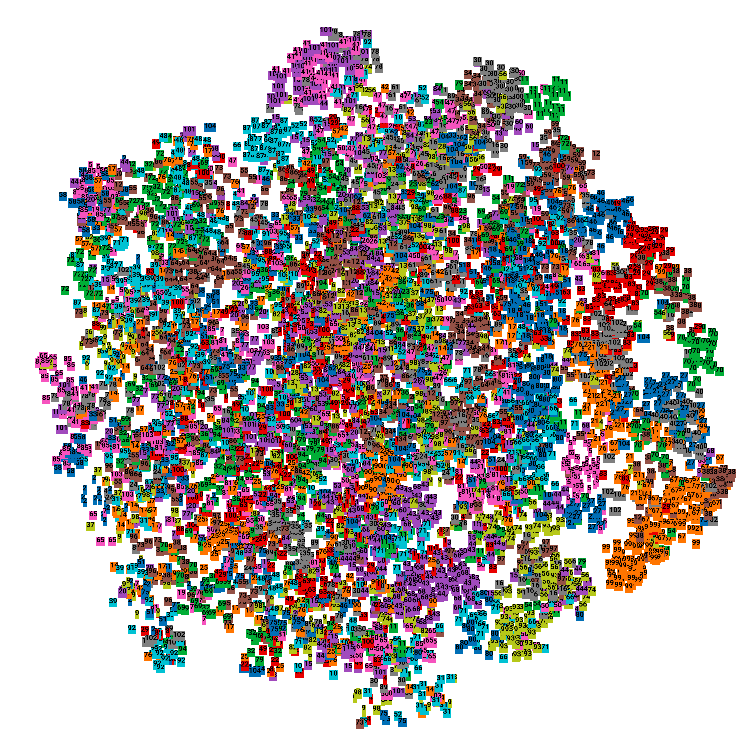
\includegraphics[width=\textwidth]{figures/untrained.png}  
  \caption{Untrained}
  \label{fig:0e}
\end{subfigure}
\hfill
\begin{subfigure}[b]{0.3\textwidth}
%   \centering
  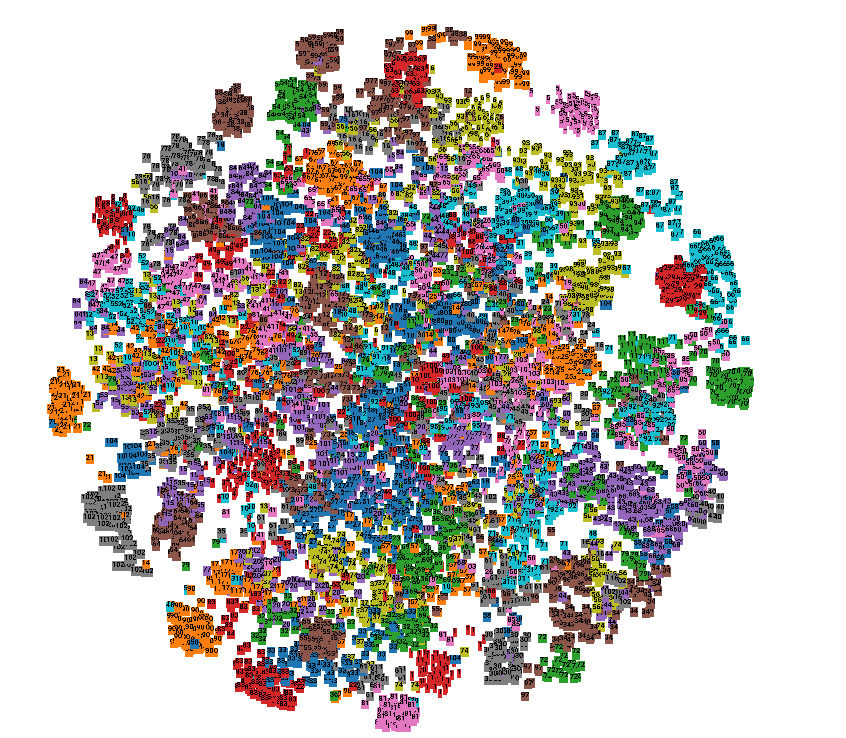
\includegraphics[width=\textwidth]{figures/5e_tsne.png}  
  \caption{After 5 Epochs}
  \label{fig:5e}
\end{subfigure}
\hfill
\begin{subfigure}[b]{0.3\textwidth}
%   \centering
  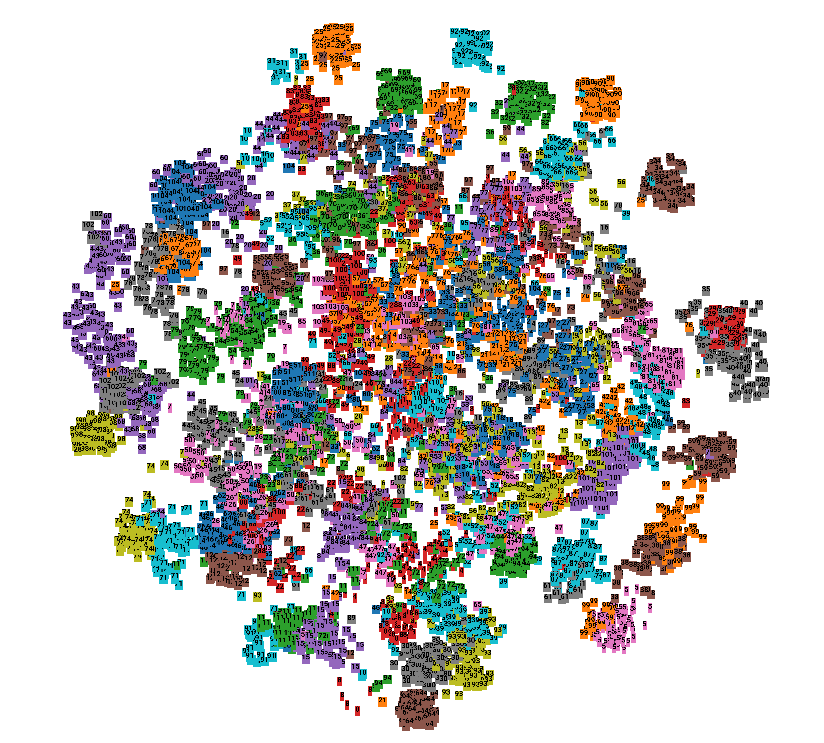
\includegraphics[width=\textwidth]{figures/full_tsne.png}  
  \caption{After 100 Epochs}
  \label{fig:100e}
\end{subfigure}
    \caption{Comparison of cluster at different instant}
    \vspace*{-\baselineskip}
    \label{fig:clusters}
\end{figure}

\begin{itemize}
    \item In Fig.~\ref{fig:0e}, we show the untrained data. It can be seen that points of similar labels are grouped together to some extent, though the clusters are not formed distinctly.
    % \vspace*{-0.4cm}

% It is a well accepted fact that the weights of the penultimate layer of the neural network represe the representation of 
% After training the classification model with the training data points for 5 epochs, we obtain the 

    \item In Fig.~\ref{fig:5e}, we show the plot formed by the learned output vectors that were taken from the last layer of the classification model after 5 epochs of the training for the same test data points. As it can be seen, on a minimalistic training, they quickly form better clusters.
    %   \vspace*{-0.4cm}
    \item At the end of training, after 100 epochs, the points form more distinct clusters as shown in Fig.~\ref{fig:100e}.
\end{itemize}

% Unsupervised Learning started
\section{Unsupervised Learning}


\subsection{Background}
Unsupervised learning is the machine learning technique that is used to train the model without labels. The clustering algorithm like KNN, K-means, hierarchical clustering, and others. 
	Learning used to happen based upon minimizing the intra-cluster distance and maximizing the inter-cluster distances. Similar data points stay near a similar point and far from the non-similar ones. This can be used for the inference of the unseen classes.
	
	As the Fig[2], given the set of unlabelled program and pass them through a  machine learning model. The model will try to form clusters of similar programs during the training. After training is done, we perform inference on the model, it try to assign the program to the best-suited cluster. This is a schematic diagram of the flow for better understanding.

	Few short learning is a way of unsupervised learning in which while inference there is some data point in which the trained model adjusts the final prediction.

\begin{figure}[t]
    \centering
    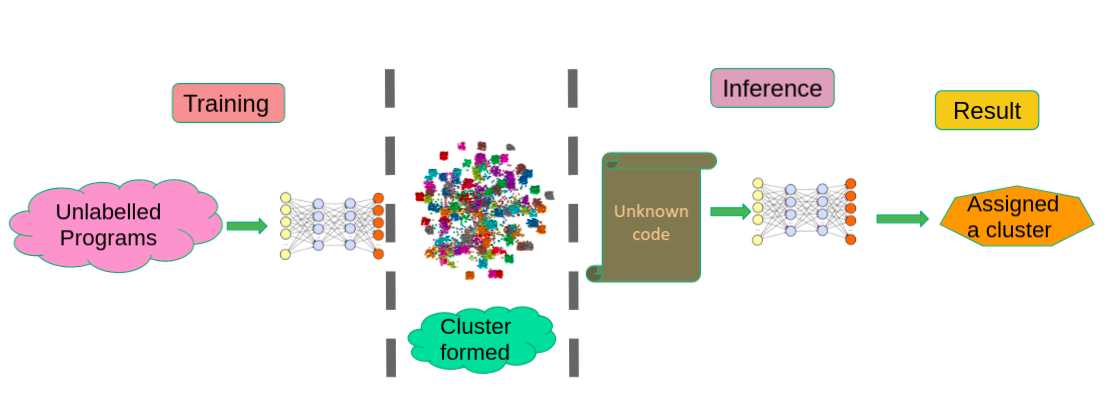
\includegraphics[scale=0.4]{figures/chapter-2/unsupervised.png}
    \caption{Algorithm Recognition in Unsupervised Way}
     \label{fig:unsupervised-background}
\end{figure}

\subsection{Few short learning}
	    It is a type of unsupervised learning, in which the training phase has two sets i.e support set and a Query set. The training happens in task. Each task consist of N classes and K datapoint in the support set and N classes in the support set. Each task has a mutually exclusive set i.e. all the N classes are not part of another task.
% 	Training

    A task is given to the model and support set is passed to the model. Now to see how much the model learns after first task, we run it on the query set for which we knew the label. The datapoint belonging to same class should lie near to each other. In the example fig[], Cat in the query set of task 1 should lie near the cat cluster of the support set and respectively for other classes.
	
	The Loss function is formulated in terms of the distance metic. If the query set is far apart during training then more is the loss and that needs to backpropagate for the better learning of the next task or batch.

\begin{figure}[t]
    \centering
    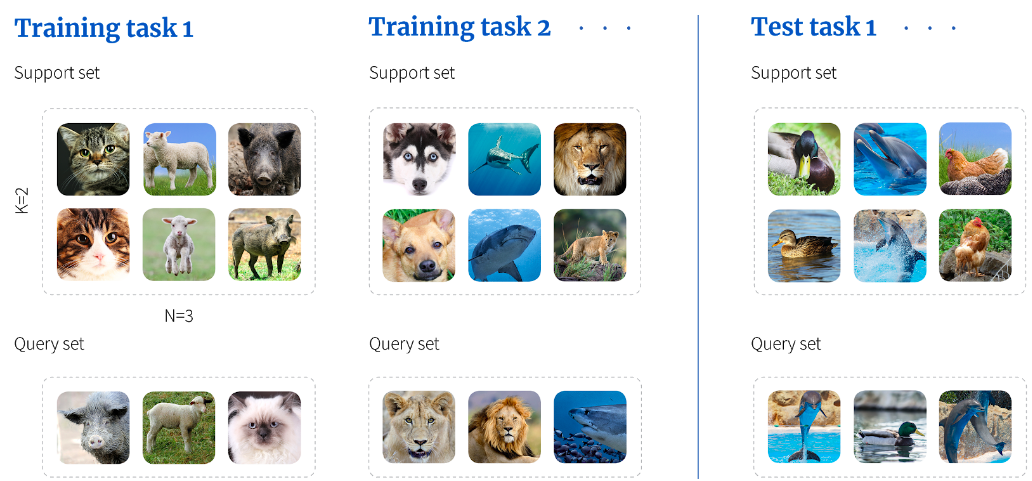
\includegraphics[scale=0.4]{figures/chapter-2/unsupervised_few_short.png}
    \caption{Few Short Learning Example}
     \label{fig:unsupervised-fewShort}
\end{figure}

\subsection{Program categorization for unseen programs}
Inspring from the work mentioned above, we want to apply the same technique to the programs. We make the required changes to the ProtoNet codebase to adapt to our work. 

\begin{figure}[t]
    \centering
    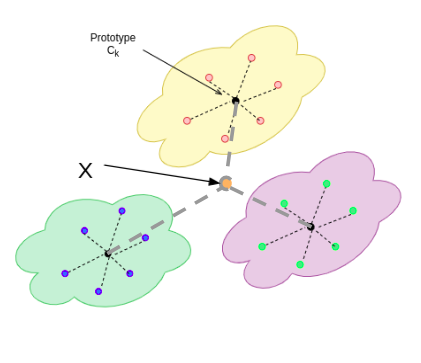
\includegraphics[scale=0.5]{figures/chapter-2/prototypes.png}
    \caption{Prototypes}
     \label{fig:unsupervised-prototypes}
\end{figure}

\subsection{ProtoNet}
\subsubsection{Prototype}
During the training phase when the support set is passed the model. Each class forms an aggregate point from other participating points and known as the prototype.
 
\subsubsection{Loss function}
During the training phase, datapoint from form each class of the Query set to evaluated against the respective prototype. The loss function forms the probability distribution of the point to which class it lies. Less is the distance, near is the point.
    		           

\subsection{Dataset}
We have selected the POJ-104 dataset\ref{} for our experiments. It has 104 type of different program which acts like class or label and each class has approximately ~500 programs. We have split this dataset into Train: Test: Val →  1-80 classes (80): 81-94 classes (14): 95-104 classes (10).

\subsection{Model Architecture}
The implementation was done using PyTorch in python. The first input layer expects a 300-dimension vector which is followed by a simple three-layered Multi-Level Perceptron(MLP) with a softmax layer for output. The Prototypical is used as the loss function and Adam optimizer. The whole training runs for 100 epochs.

\subsection{Results}

\begin{table}[h]
\begin{tabular}{lllll}
\hline
\multirow{2}{*}{\textbf{POJ Experiment}} & \multicolumn{2}{l}{\textbf{5 ways}} & \multicolumn{2}{l}{\textbf{10 ways}} \\
 & \textbf{1 Shot} & \textbf{5 Shot} & \textbf{1 Shot} & \textbf{5 Shot} \\
\hline
Test Accuracy \% & 78.47 & 89.66 & 80.9 & 91.27 \\
\hline
\end{tabular}
\centering
\caption{Compare the accuracy percentage.}
\label{unsupervised-acc}
\end{table}
\chapter{Distribution And Fusion Case Study}
\label{chap:ch4}

\begin{figure}[t]
    \centering
    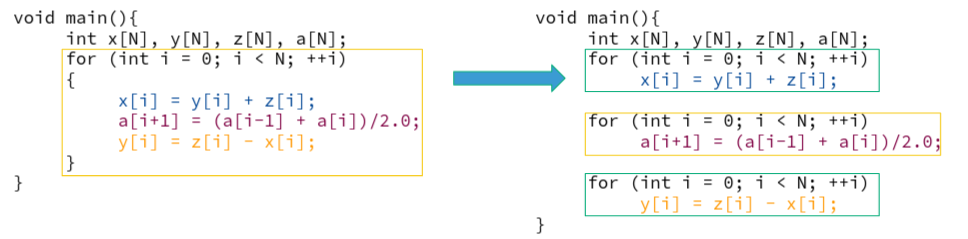
\includegraphics[scale=0.45]{figures/chapter-4/distribution_introduction.png}
    \caption{Distributed Loops}
     \label{fig:dist-introduction}
\end{figure}

\section{Background}
    The optimization in the compiler is very important of code generation.
Good is the optimization, better is the code execution. Here, we will talk about Loop Distribution optimization.

    In Loop Distribution, the bigger loop is split into smaller loops as shown in Fig.~\ref{fig:dist-introduction}. It may lead to improved loop vectorization and better locality. In LLVM, the loop distribution is not efficient, heuristic-based and does not promise the optimal distribution. It lead to miss in the vectorization opportunities.

\section{Introduction}
We want to have a ML based Loop Distribution optimization in the LLVM. It could overcome the flaws of the existing Loop Distribution. But in this chapter, we will discuss about Frontier Pass and it's importance.

\begin{figure}[t]
    \centering
    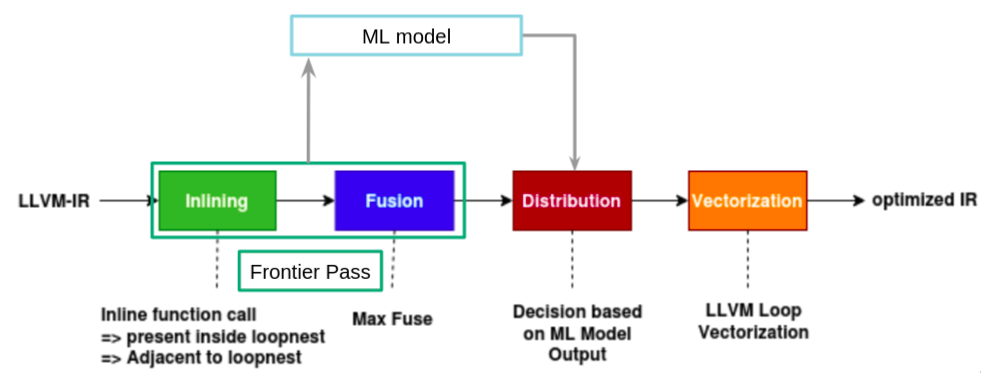
\includegraphics[scale=0.4]{figures/chapter-4/distribution_flow.png}
    \caption{Position of Frontier Pass in the workflow}
     \label{fig:dist-flow}
\end{figure}

\section{Frontier Pass}\label{sec:distribution:fp}
 We have proposed a pass sequence of custom inlining followed by fusion. See the Fig.~\ref{fig:dist-flow}. We have written loop-function-inline pass, which pass through loop and try to forcefully inline the function inside the innermost loop as well as at the same level of the loop. After performing loop-function inlining, we have enable the fusion pass in the pipeline. The loop fusion is the reverse of loop distribution. The fusion combined multiple loop to form a big loop. 
 
%  The selected loop should not have any control flow  and call instruction inside it.


%  For the Bigger picture to happen, we have a design proposal that only innermost loop will be selected.
\section{Ideology Behind Frontier Pass}
To achieve the optimal distribution, we first want to have max distribution. The max distribution can be achieve from max fusion. As per the sec~\ref{sec:distribution:fp}, we have added fusion to the pipeline. For better fusion opportunities, some custom inlining can be helpful. We have developed loop-function-inline as mentioned in Sec.~\ref{sec:distribution:fp} and schedule it in the LLVM pass sequence. 

\begin{table}[h]
\begin{tabular}{|l|l|l|}
\hline
\multirow{2}{*}{\textbf{BENCHMARK}} & \multicolumn{2}{c|}{\textbf{\#Candidates for Loop Fusion}} \\ \cline{2-3} 
 & \textbf{O3-Fusion} & \textbf{O3-Frontier Pass} \\ \hline
blender\_r & 3952 & 7042 \\ \hline
deepsjeng\_r & 94 & 244 \\ \hline
imagick\_r & 2735 & 3065 \\ \hline
lbm\_r & 8 & 8 \\ \hline
leela\_r & 53 & 69 \\ \hline
mcf\_r & 14 & 16 \\ \hline
namd\_r & 1392 & 1812 \\ \hline
omnetpp\_r & 203 & 2200 \\ \hline
povray\_r & 229 & 2232 \\ \hline
x264\_r & 356 & 760 \\ \hline
xalancbmk\_r & 1017 & 1147 \\ \hline
xz\_r & 67 & 85 \\ \hline
\end{tabular}
\centering
\caption{Candidates for Loop Fusion}
\label{tab:dist:fuscand}
\end{table}

\section{Case Study}
In this section, we will see the effect of the frontier pass on the fusion candidates and runtime. We have run our xperimentation on the SPEC 2017 benchmark and  observe the fusion candidate. Here, we are comparing the metrics between the O3 optimization with fusion enabled and O3 optimization with Frontier Pass.

\subsection{Fusion Candidate}
Here, we are comparing the \# Candidates for Loop Fusion between the O3 optimization with fusion enabled and O3 optimization with Frontier Pass. See the Tab.~\ref{tab:dist:fuscand}. Incase of Frontier Pass, there are more fusion candidates which are better for max fusion. Hence frontier pass is important part of the ML-based loop distribution as the prepossessing step. 

\subsection{Runtime}
Here, we are comparing the runtime between the O3 optimization with fusion enabled and O3 optimization with Frontier Pass. See the Tab.~\ref{tab:dist:fpruntime}. Due to Frontier Pass,  they is not much overhead added to the runtime and they are some positive cases where there is improvement in runtime.



% Please add the following required packages to your document preamble:
% \usepackage{multirow}
\begin{table}[h]
\begin{tabular}{|l|l|l|}
\hline
\multirow{2}{*}{\textbf{BENCHMARK}} & \multicolumn{2}{c|}{\textbf{Runtime in seconds}} \\ \cline{2-3} 
 & \textbf{O3-Fusion} & \textbf{O3-Frontier Pass} \\ \hline
blender\_r & 298 & 311 \\ \hline
deepsjeng\_r & 343 & 336 \\ \hline
imagick\_r & 440 & 437 \\ \hline
lbm\_r & 544 & 545 \\ \hline
leela\_r & 503 & 498 \\ \hline
mcf\_r & 542 & 530 \\ \hline
namd\_r & 234 & 239 \\ \hline
omnetpp\_r & 636 & 602 \\ \hline
povray\_r & 459 & 439 \\ \hline
x264\_r & 422 & 284 \\ \hline
xalancbmk\_r & 407 & 392 \\ \hline
xz\_r & 303 & 442 \\ \hline
\end{tabular}
\centering
\caption{Runtime Overhead}
\label{tab:dist:fpruntime}
\end{table}

\section{Model}
 The generated graphs are used as inputs in our modeling pipeline. In this section, we explain how we represent SDGs using IR2Vec representations and the way we model the reinforcement learning model to consume this information using Gated Graph Neural Networks. We also discuss various parameters of the model, including the design of our cost model, with which we arrive at a relative number of clock ticks that take into account impact by both locality and vectorization.

% CONSTRAINTS ON SDG
% TOPOLOGICAL MATH FORMULATION
% MERGE AND DISTRIBUTE

\subsection{GGNN based reinforcement learning model}
    Fig. 2 shows the workflow of the reinforcement learning model for our problem. The model takes SDG as input and maps it to a GGNN. The IR2Vec embeddings take the type of operation, a variable is involved into consideration.

    GGNN[Y Li] is the upgradation of the graph neural network by adding an Gating mechanism using the Gated Recurrent Units  and unroll the recurrence
for a fixed number of steps T. Each node of the GGNN has a hidden presentation which is initially represented using IR2Vec embeddings and dannotation vectors. 

In our work, we use the propagation model of the GGNN to get the updated hidden state vectors at any instance of time, 

Initial Presentation 
hno = IR2vec Embedding according to SDG node   
Hn0 : [hno:Ano]  
A is the meta vector [isStartNode, IsVisited]
Ano  = [0,0]  as no node visited in the starting

At any instant t for node n
Hnt-1 : [hnt-1:Ant-1]
f : Hnt-1 → hant-1 
% x :  ∑n’ e neigh(n) han’t-1 + b
hnt	 : GRU(hant-1,, x)

Using this mathematical calculation, we are updating the hidden nodes.
 
    The set of all possible visitable nodes at the start of the topological walk is the initial state of the environment. The mode takes the merge decision from the set of legal node choices given by topological walk on GGNN. The agent makes a decision to which node to visit and after visiting, what subsequent action should be taken(merge, distribute). For new node visited we updated the annotation isVisited to True. If subsequent decision is merge, then we update the GGNN with a new edge called ‘Merge Edge’ and is placed  between the source and visited node. If subsequent decision is distribute, we do not apply any change to the GGNN structure. Then we perform propagation on the GGNN to update the hidden state of the nodes. We continue this till all the nodes are visited.

\subsection{RL Model}
Parameters of RL Model → State, action, reward
We are trying to represent our problem as the Markov decision Problem. We try to solve this problem using the reinforcement learning setting. We convert the SDG graph to GGNN and get the state of the environment at any instance of time. We are trying to solve this problem in partial observable space. 

\paragraph{State} It is the presentation of the environment at an instant of time. We are using GGNN to capture the state of the environment.
Si = ({Set of all the possible visitable Nodes from the current node}) 
Here we have added a constraint that nodes are selected as per the topological walk.   

\paragraph{Initial state} At the start point, the state will be all the set of all the possible visitable Nodes..
Si = ({Set of eligible Node}, focusNode) focusNode=None 

\paragraph{Action} 
Given a state, select the next node in the graph to be visited by the graph followed by the merge or distribute decision. This is constrained by the topological sort to maintain the legality of the program.
If no node visited till now:
	A = (select nextnode from state)
else
% A = (select nextnode from state, D \ɛ {Merge distributed})
After action is taken, we update the environment and get the next state.

\paragraph{Reward} For every action, the environment gives back a feedback which is called reward. It signifies the goodness of the action. In our work, we are using a static cost model sec 3.6 to calculate the reward by using the formulae LCo-LCd/LCo(where LC is the LoopCost). We use reward based on the loopCost at the end of the topological walk and for the intermediate action, we give zero as reward. The negative reward signifies that the distributed loop is not efficient. In RL, we want to maximize the rewards.

	Use DQN Algorithm to perform training the 1980 loops. The batch size of 64 with replay buffer size of 10000. To introduce  exploration in the training, we gradually decrease the epsilon with time. 

\chapter{Machine Learning Framework for Register Allocation}
\label{chap:ch5}

\section{Background}
Register Allocation is an old and classic optimization problem. Many researchers provide many solutions for it but all are heuristically defined. In a heuristical problem, it depends upon the developer’s domain expertise. There would be a possibility that some important heuristics are missed and may lead to suboptimal performance.

The allocation should be done efficiently as the number of the registers is limited in number and may lead to poor performance if the register does not give to a memory-bound variable. This leads to an increase in the use of the memory-based load and store operation and these are more expensive than the register operations. 

The popular register allocations are greedy, basic, fast, and PBQP register allocation. In this we are interested in the register allocation via Interference graph coloring. In the fig[1], there is a sample code for which we have the live interval interference chart. The Live interval are the scope of the variable when the variable was first defined and last used. Every variable has it own live interval and those may interfere with others. We can formulate this problem as the graph color program where the node is the variable or live interval and edges are the inference among the nodes. The rule for the thumb, no two adjacent nodes be assigned the same color(register). The optimal graph coloring is a classic NP-Hard problem. 

The LLVM has Greedy and Basic allocators based on the graph coloring. There are four strategies used by these allocators respectively namely Splitting, Coalescing, eviction, and spilling. 

\paragraph{Splitting} - In this a selected node or live of the graph is divided into two sub-live intervals depending upon the point of the splitting. The newly created live interval may or not form the edge between the existing nodes.

\paragraph{Coalescing} - In these two nodes which have the same variable value can be combined to form one node or live interval. 
\paragraph{Eviction} - if some node of the graphs is already assigned a colored, but we wanted to uncolor the respective node. This process is known as eviction.
\paragraph{Spilling} - If the allocator ran out of register or heuristically suggests assigning the variable to the memory. Memory load-store are costlier operations.

\begin{figure}[t]
    \centering
    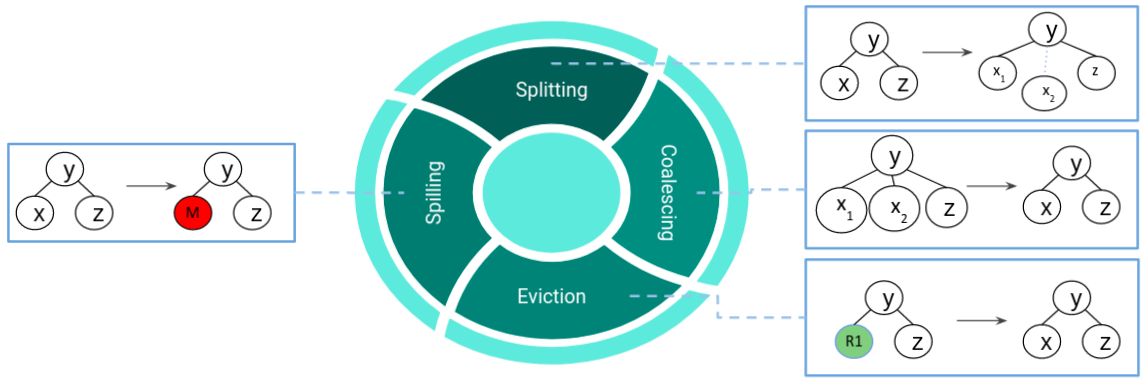
\includegraphics[scale=0.4]{figures/chapter-5/mlra_strategies.png}
    \caption{Register Allocation - Strategies}
     \label{fig:mlra-strat}
\end{figure}

The \textit{greedy allocator} uses all the four strategies in a heuristic manner and \textit{Basic allocator} uses splitting and spilling.

The current allocators are heuristically defined and provide sub-optimal solutions. Machine learning could help to better solutions.

\section{Previous Work}
The register allocation using deep learning [D.Das at el 2020]. In this, they tried to use the Bi-LSTM based deep learning model to predict the color or register to allocated. The graph as input to a model of max size 100 nodes and node has hidden representation as a bit vector of size 100. The bit index is set to one when the node interference with the respective node in the graph. 

But there were several drawbacks to their work. The solution was not integrated back to the LLVM pipeline. The proper modeling of the interference rule was not done due to which predict adjacent nodes are assigned the same color and lead to incorrect register assignments. They have added a correction phase to overcome this problem. The dataset used for the training was not realistic as it was sampled from random graphs using the nauty api[].

\section{Introduction}
We have developed a Machine learning framework for register allocation. We have divided the framework into 3 components- Capture Interference graph, ML model interface, Code generation, and multi-architecture support. The communication between the Capture interference graph, ML model, and code generation is done via GPRC.

The GRPC is a medium for cross-platform communication between C++ (LLVM) and Python (ML Model)

\begin{figure}[t]
    \centering
    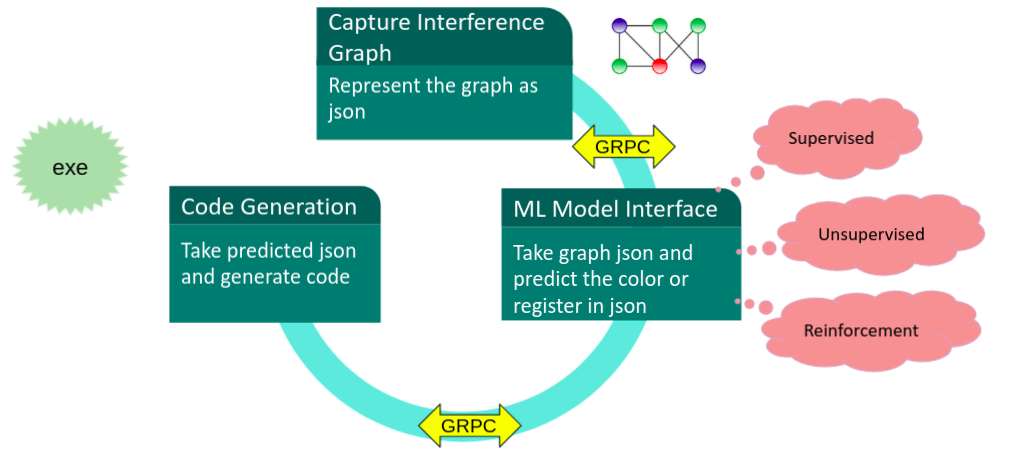
\includegraphics[scale=0.4]{figures/chapter-5/mlra_components.png}
    \caption{Components of correct ML based register allocation}
     \label{fig:mlra-components}
\end{figure}

\section{Framework Components}
\subsection{Capture Interference Graph}
We have written a pass in LLVM which is responsible for capturing the inference graphs for the given input files. We annotate the graph with more information which would be later used by the other components.

The node comprises of Node label, information regarding type of register physical or virtual, Color and register Id if physical register, the class of the register, and embedding representation.

\begin{figure}[t]
    \centering
    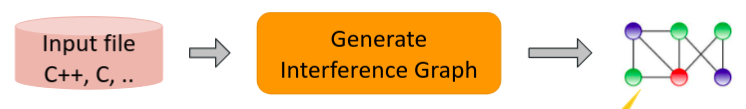
\includegraphics[scale=0.4]{figures/chapter-5/mlra_cig.png}
    \caption{Capture interference graphs}
     \label{fig:mlra-cig}
\end{figure}

The edge or interference that we are considering are between Virtual register and virtual register and between virtual register and virtual register. There are some physical register which are already in used and can’t be used and to respect the interference rule, the edge is added. The Virtual -- virtual is the base edge.
\subsection{ML Model interface}

\subsubsection{Training}
From the previous component, we got the interference graphs and pass to the training paradigm. The interference graph goes to the model in th python where it request to start the server to the LLVM through the GPRC. After the server got started, the ML model run and share its prediction with the codegen through another GRPC call and codegen sends some information back to the model for further execution. 

\begin{figure}[t]
    \centering
    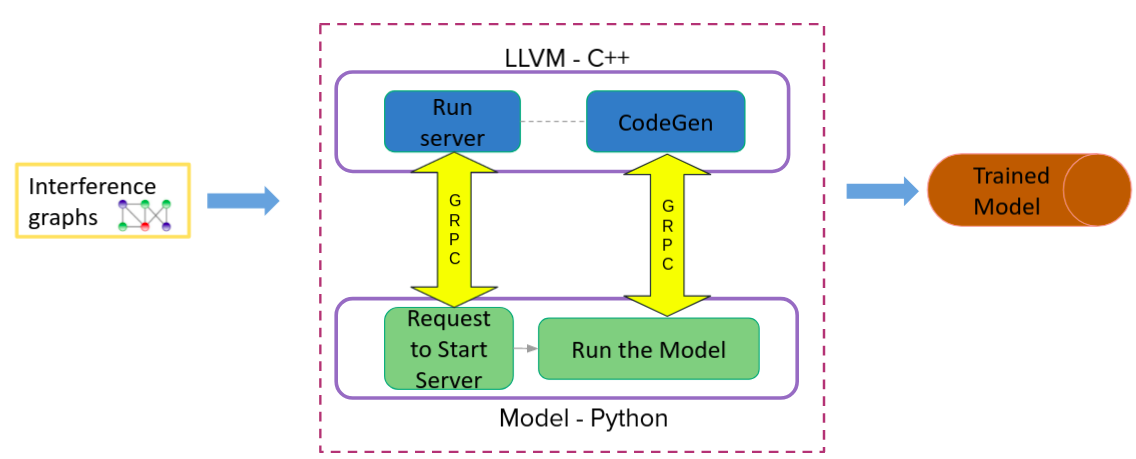
\includegraphics[scale=0.4]{figures/chapter-5/mlra_training.png}
    \caption{Train the model using the GRPC}
     \label{fig:mlra-training}
\end{figure}

After all the interference graphs are visited, training is finished and the trained model used for the inference.
\subsection{Code generation or inference}
After the model is trained, we have added the integrated model with LLVM so that code generation could be done using the prediction suggested by the configured trained model.

While inference,the input file is given the LLVM and in the pipeline,  capture interference graph pass is invoke and the graph is then send to the Python through GRPC where it is feed to the trained model. The trained model send a color prediction json to the LLVM. In LLVM, the predicted colors/registers are mapped to the virtual registers and code is generated. 
\begin{figure}[t]
    \centering
    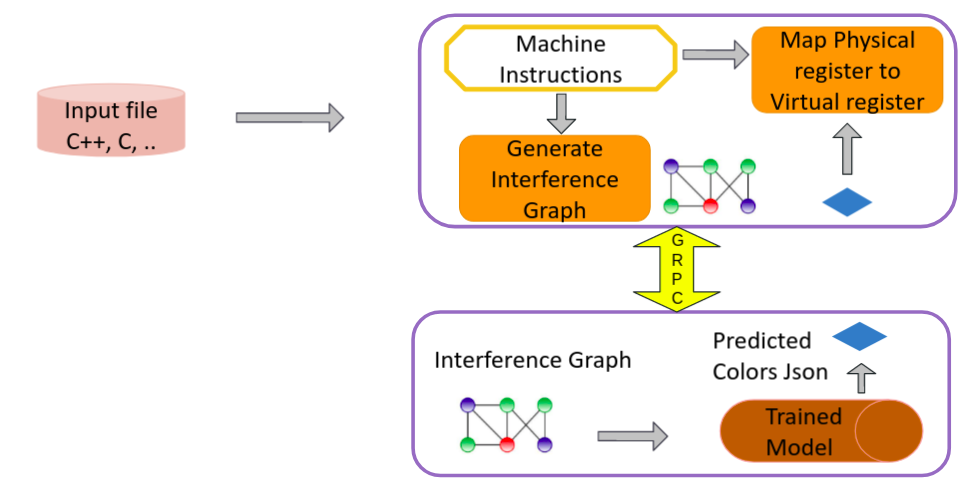
\includegraphics[scale=0.4]{figures/chapter-5/mlra_inference.png}
    \caption{Code generation using the trained model}
     \label{fig:mlra-inference}
\end{figure}
\section{Architecture}
Different backends have their own instruction set and register set. In LLVM, this information is managed by TD files. TableGen takes the TD files and applies them to the backend so that this information is available at the code generation.

The TD files consist of information regarding different types of registers, classes information to which the register belongs, aliasing information, sub-registers details, and many more.
We have implemented a pass that captures information from the TD files and generates the configuration files which are used in different components. In the pass, we can configure the classes of the registers which we want to support, mapping between the color and the registers and overlapping information of the subregisters. 

These configuration files are used in the capture interference graph component to get the register id, color, register classes and other information. In the ML model inference, overlapping information, register color mapping configuration is used. Similarly in the code generation, color register mapping is used to get the color corresponding to the register.

\section{Correctness Results}
To check the correctness of work framework, we have chosen GCC Torture benchmark. It is also part of llvm-testsuite. GCC Torture is a stress testing benchmark. For the experimentation, we have selected 1483 input files. We have selected two architectures X86 and AArch64 and successfully generated the code followed by successful execution.

For AArch64, we used QEMU to run the generated code on X86 machine. QEMU is a simulator or virtualization software that provide the libraries needed by assembly code of different architecture and executing on others.

% Please add the following required packages to your document preamble:

\ref{tab:correction} 

\begin{table}[h]
\begin{tabular}{llllll}
\hline
\textbf{Architecture} & \textbf{\begin{tabular}[c]{@{}l@{}}Program \\ files\end{tabular}} & \textbf{\begin{tabular}[c]{@{}l@{}}Base \\ compilable files\end{tabular}} & \textbf{\begin{tabular}[c]{@{}l@{}}Assembly\\ files generated\end{tabular}} & \textbf{\begin{tabular}[c]{@{}l@{}}Binary \\ files generated\end{tabular}} & \textbf{\begin{tabular}[c]{@{}l@{}}Successful \\ execution\end{tabular}} \\ \hline
\textbf{X86} & 1483 & 1483 & 1483 & 1483 & 1483 \\ \hline
\textbf{\begin{tabular}[c]{@{}l@{}}AArch64\\ (QEMU)\end{tabular}} & 1483 & 1479 & 1479 & 1479 & 1479 \\ \hline
\end{tabular}
\centering
\label{tab:correction}
\end{table}

The errors undertaken will evaluating the framework are code generation error, linking error, runtime error, and semantic errors. A lot of iteration went into fixing these errors. We were able to achieve zero errors.

\begin{table}[h]
\begin{tabular}{lllll}
\hline
\textbf{Architecture} & \textbf{\begin{tabular}[c]{@{}l@{}}Code \\ generation error\end{tabular}} & \textbf{Linking error} & \textbf{\begin{tabular}[c]{@{}l@{}}Runtime\\ error\end{tabular}} & \textbf{Semantic error} \\ \hline
\textbf{X86} & 0 & 0 & 0 & 0 \\ \hline
\textbf{AArch64} & 0 & 0 & 0 & 0 \\ \hline
\end{tabular}
\centering
\end{table}

\section{MLRA in Action}
Here we want to show how the framework can be used to register prediction using a naive reinforcement learning model on X86 architecture. We have taken 50K interference graphs from the SPEC 2017 benchmarks. Embedding are generated using the IR2Vec on machine instructions representation(MIR). We are using reinforcement learning as the ML model interface and the objective of the model is to minimize the spill cost.

The spill cost is the weight associated with each variable. Higher the value of spill cost more costly is load-store memory operations.

\begin{figure}[t]
    \centering
    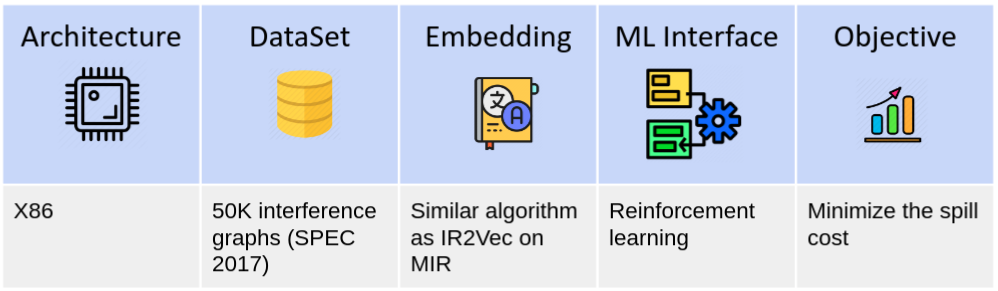
\includegraphics[scale=0.45]{figures/chapter-5/mlra_action.png}
    \caption{Framework configurations}
     \label{fig:mlra-fw}
\end{figure}

\subsection{Reinforcement Learning Model}
Implemented a policy using the DQN algorithm in that the agent predicts which node should be assigned the register first.  While assigning the register, the policy is constraint by the interference rule. The objective of the model is to minimize the spillcost.

\subsection{Results}

Run the inference with trained model and showed our results on PolyBench and MiBench.
\subsubsection{PolyBench}
It is a Loop benchmarks which have different computational intensive programs.

\begin{figure}[t]
    \centering
    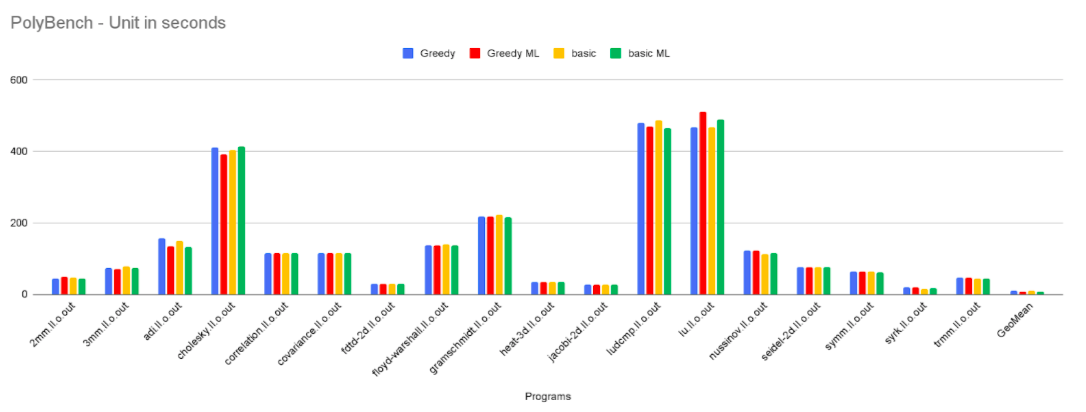
\includegraphics[scale=0.4]{figures/chapter-5/polybench.png}
    \caption{PolyBench - Runtime}
     \label{fig:mlra-polybench}
\end{figure}


\begin{table}[h]
\begin{tabular}{|l|l|l|l|l|}
\hline
 & \textbf{Greedy} & \textbf{Greedy ML} & \textbf{Basic} & \textbf{Basic ML} \\ \hline
GeoMean & \multicolumn{1}{r|}{9.306} & \multicolumn{1}{r|}{9.050} & \multicolumn{1}{r|}{9.259} & \multicolumn{1}{r|}{8.891} \\ \hline
\end{tabular}
\centering
\end{table}

\subsubsection{MiBench}
This Benchmark is a micro-kernel benchmarks which are suitable for embedded device.

\begin{figure}[t]
    \centering
    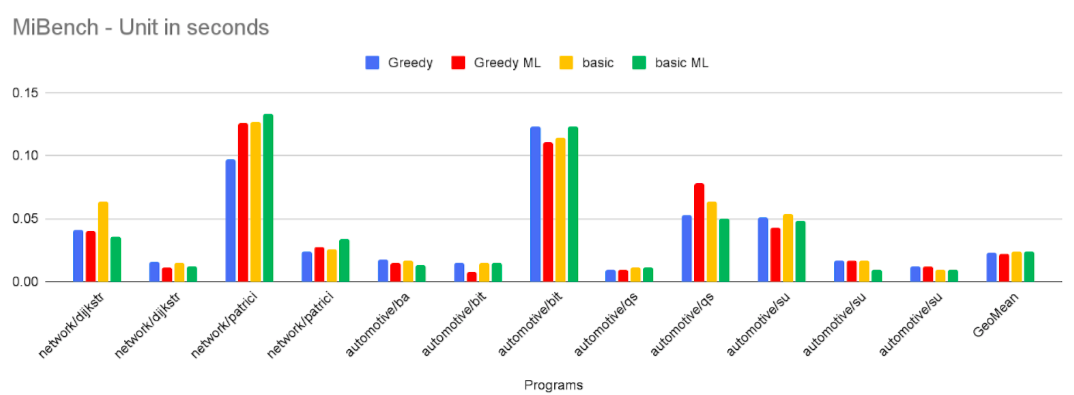
\includegraphics[scale=0.4]{figures/chapter-5/MiBench.png}
    \caption{Runtime - MiBench}
     \label{fig:mlra-mibench}
\end{figure}

\begin{table}[h]
\begin{tabular}{|l|l|l|l|l|}
\hline
 & \textbf{Greedy} & \textbf{Greedy ML} & \textbf{Basic} & \textbf{Basic ML} \\ \hline
GeoMean & \multicolumn{1}{r|}{0.0227} & \multicolumn{1}{r|}{0.0220} & \multicolumn{1}{r|}{0.0242} & \multicolumn{1}{r|}{0.0237} \\ \hline
\end{tabular}
\centering
\end{table}
\chapter{Conclusion and Future Directions}
\label{chap:conclude}

% Conclude your thesis.

In Chap XXX

In \textbf{Chapter~\ref{chap:ch2}}, We are able to achieve better results with respect to the prior work in term of both accuracy. Additionally, the training time of the model is far better then the others. \newline

In Chap XXX

In \textbf{Chapter~\ref{chap:ch3}}, We successfully generates the vector presentation using IR2Vec for the POJ/OJ Dataset. Using this representation and the without any complex model architecture, we are able to get better results than the previous work for the supervised learning setting. On the other hand for unsupervised learning, we are  able to cluster the unseen classes which were not the part of the training dataset.

This work would be extended to classify or identify the binaries files. \newline

In Chap XXX

In \textbf{Chapter~\ref{chap:ch4}},, We have developed a Frontier pass in LLVM which perform loop-function inlining followed by fusion. We have done a Case study and are able show the requirement of the Frontier Pass for the Machine Learning Based Loop Distribution. \newline

In Chap XXX \newline

In \textbf{Chapter~\ref{chap:ch5}}, We show that We have successfully developed a framework for register allocation which generates semantically correct code, which supports multiple architectures, and which can communicate between LLVM (in C++) and ML model (in Python).

This framework can also be used to support the ML based optimizations in LLVM for other optimization problems, in which such kind of information to-from is required.

\clearpage
\newpage
\addcontentsline{toc}{chapter}{References} % Please do not remove this
% \addtocontents{toc}{\setcounter{tocdepth}{1}} 
\bibliographystyle{alpha}
%%\bibliographystyle{iiththesis}
\bibliography{references}
\end{document}
